\documentclass{article}
\usepackage[utf8]{inputenc}
\usepackage{graphicx}
\usepackage{caption}
\usepackage{hyperref}
\usepackage{tcolorbox}
\tcbuselibrary{theorems}

\newenvironment{myminipage}[1]{\minipage{#1} 
 \captionsetup{width=\textwidth, name=Fig., labelfont={it,bf}}
 }{\endminipage} 

\newtcbtheorem[no counter]{need}{Need}%
{ 
  sharp corners,
  colback=green!5,
  colframe=green!25,
  fonttitle=\bfseries,
  coltitle=black,
 }{th}

\begin{document}

\begin{center}

\includegraphics[width=\textwidth]{Data/logocircle.png}
\title{Relazione greenLivery}
\author{Flavio, Nicola, Luca, Matteo, Mario}
\end{center}
\renewcommand{\contentsname}{Indice}

\maketitle
\tableofcontents

\section{Introduzione}\par
Il topic del progetto dato dal docente è la realizzazione di un servizio legato a cibo e alimentazione. Con particolare aree di interessi,come: \par
\begin{itemize}
    \item \textbf{dieta}:gestione dieta per uno stile di vita sano, e.g., per motivi medici/altro, dieta per sportivi, gestione ricettari, diario della dieta \par
    \item \textbf{green}:cambiamento abitudini alimentari, diminuzione di food-waste e risorse impiegate (e.g., per produrre carne), gestione smart di coltivazioni e allevamenti \par
    \item \textbf{cultura}: tradizioni alimentari, prodotti tipici del territorio, percorsi enogastronomici, slowfood\par
    \item \textbf{aggregazione/commercio}: ristoranti, bar, delivery della spesa o di piatti pronti \par
    \item \textbf{tecnologia}: tele-dining (e.g., aperitivo da remoto), mukbang (guardare altri mangiare su YouTube), food printing, ... \par
\end{itemize}
\vspace{1cm}



    \addcontentsline{toc}{subsection}{\numberline{1.1}Argomento del progetto} \par
    \numberline{\fontsize{4mm}{1mm}\selectfont \textbf{1.1 Argomento del progetto}}\vspace{0.5cm}
    L'obiettivo del nostro progetto "Greenlivery" è sviluppare un'app di delivery che si concentra sulla sostenibilità e combattere il food waste. La nostra app offre la possibilità di ordinare cibo da ristoranti locali con consegne effettuate in modo eco-compatibile, contribuendo così a ridurre l'impatto ambientale delle consegne. Inoltre, siamo sensibili allo spreco alimentare rendendo soddisfatti sia i clienti che i ristoranti, i quali possono utilizzare la nostra app per ridurre il loro spreco alimentare, in modo da poter ridurre i costi e aumentare i profitti con la vendita di "Food Magic Box".
    \vspace{1cm}
    
    \addcontentsline{toc}{subsection}{\numberline{1.2}Analisi app competitor} \par
    \numberline{\fontsize{4mm}{1mm}\selectfont\textbf{1.2 Confronto con app simili}}\vspace{0.5cm}
    Analizzando le principali app di food delivery è emerso che: tutte posseggono sia un sito web che un'app per smartphone, ci permettono di geolocalizzare il nostro indirizzo e ci consigliano i ristoranti.
    Abbiamo individuato le seguenti app competitor:
\begin{itemize}
        \item \textbf{App n1 - \href{https://www.justeat.it}{JustEat}:} Ha un’interfaccia intuitiva, con le categorie e la ricerca in primo piano, non permette però di visualizzare il nome, la foto del rider. Non consente, inoltre, di chattare con esso o con il ristorante.

        \item \textbf{App n2 - \href{https://glovoapp.com/it/it/}{Glovo}:} Ha un'interfaccia divisa in macrocategorie che ci offre servizi concorrenziali, come inviare pacchi da un indirizzo all’altro o ordinare farmaci. É possibile visualizzare delle informazione sul rider come la posizione in tempo reale e parlarci tramite live chat. Offre anche la possibilità di accumulare credito sull’app invitando degli amici ad iscriversi. É possibile inoltre recensire il ristorante, l’ordine ricevuto e il rider che lo ha consegnato.

        \item \textbf{App n3 - \href{https://deliveroo.it/it/}{Deliveroo}:} Come JustEat ci offre in homepage le varie categorie, le promozioni in corso e la ricerca dei ristoranti. Ci permette di visualizzare informazioni e posizione del rider ed ha un servizio di recensione come quello di Glovo. La peculiarità di questa app è poter aggiungere alcuni ristoranti tra i preferiti e visualizzarli facilmente tramite un pulsante in homepage. Aprendo le categorie è possibile filtrare i ristoranti in base a regimi alimentari (Vegano, senza glutine, kosher ...).

        \item \textbf{App n4 - \href{https://www.ubereats.com/it}{UberEats}:} Schermata intuitiva ma con meno categorie presenti rispetto ai competitor. Offre la possibilità di visualizzare tutte le info e la posizione del rider in tempo reale, ci permette inoltre di recensire non solo il ristorante e il rider, ma anche singolarmente ogni prodotto dell’ordine che abbiamo fatto.

    

\end{itemize}Abbiamo la conferma delle app competitor conosciute da parte degli utenti che hanno risposto al nostro form, nel seguente modo:
\begin{center}
    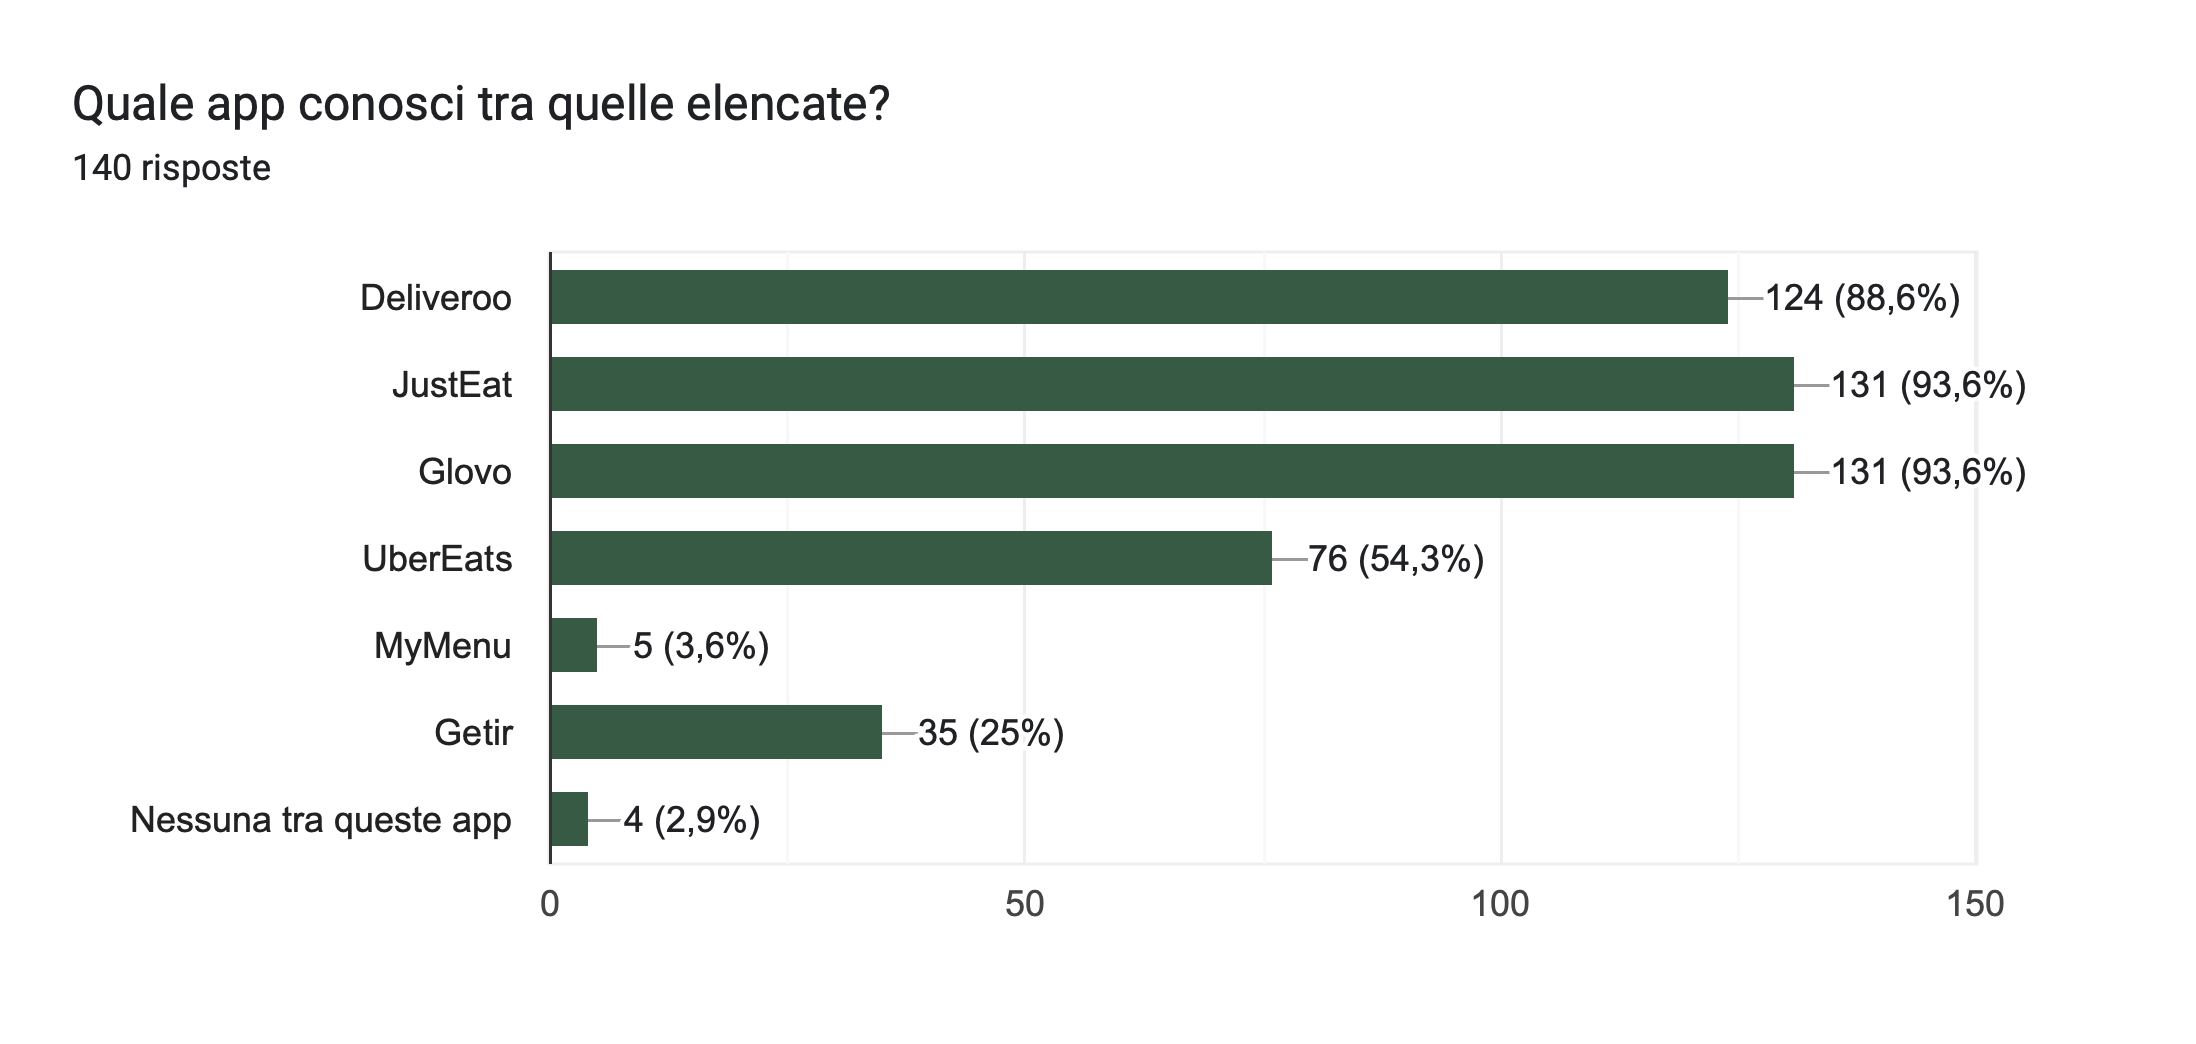
\includegraphics[width=\textwidth]{Data/Grafici/App_competitor.png} 
    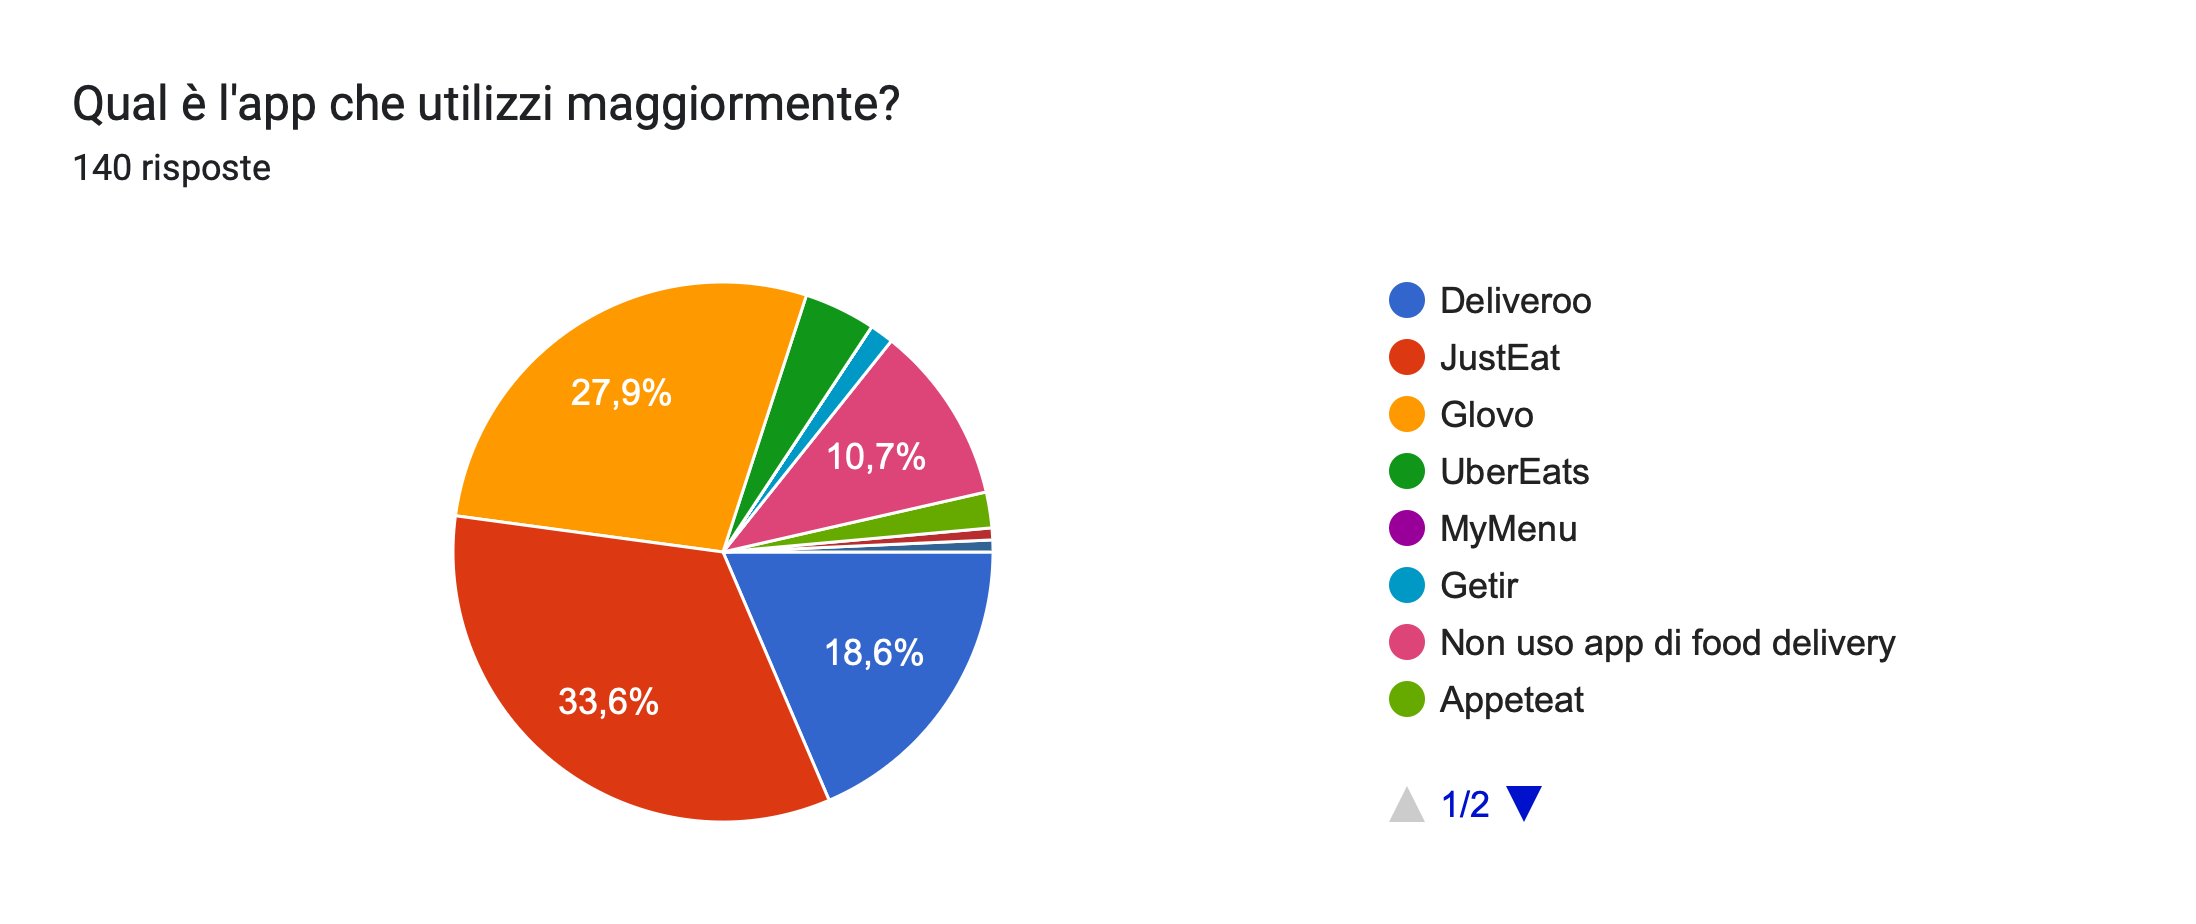
\includegraphics[width=\textwidth]{Data/Grafici/App_competitor_utilizzate.png}
\end{center}



    \vspace{1cm}
\section{Needfinding} 
In questa fase di sviluppo l’obiettivo è comprendere le necessità degli utenti per capire le funzionalità da implementare nell’applicazione. Per farlo abbiamo utilizzato due metodi: il questionario e le interviste.
    \vspace{1cm}
    \addcontentsline{toc}{subsection}{\numberline{2.1}Interviste} \par
    \numberline{\fontsize{4mm}{1mm}\selectfont \textbf{2.1 Interviste}}\vspace{0.5cm}
\par Abbiamo realizzato due versioni delle interviste, dopo aver sottoposto gli intervistati alla prima versione abbiamo trovato le criticità ed abbiamo sviluppato la versione due con domande rielaborate e più comprensibili. \par Le interviste sono state poste per lo più a colleghi di università, amici e colleghi di lavoro per una durata media di 7 minuti.\par
\par Il file con le interviste è disponibile \textbf{\href{https://wind-blob-6b0.notion.site/Interviste-de02a85b8b634f7687534d2064010b4a}{a questo sito}.}\par
  \vspace{1cm}\addcontentsline{toc}{subsubsection}{\numberline{2.1.1}Domande}\par
    \numberline{\fontsize{4mm}{1mm}\selectfont \textbf{2.1.1 Domande}}\vspace{0.5cm}
    \begin{enumerate}
    
     \item \textit{Ordini mai a domicilio?}
        \begin{enumerate}
            \item Se no, perché?
        \end{enumerate}
     \item \textit{Conoscete e avete mai utilizzato un'app di food delivery?}
     \begin{enumerate}
         \item Quali?
         \item Quanto spesso le usi?
     \end{enumerate}
     \item \textit{Quali funzionalità preferisci dell'app che utilizzi?}
     \item \textit{Quali potrebbero essere delle funzionalità che ti potrebbero tornare utilizzi ma che non sono implementate?}
    \item \textit{Ti farebbe comodo conoscere i valori nutrizionali(calorie, proteine, carboidrati, grassi) delle pietanze che ordini?}
    \begin{enumerate}
        \item La troveresti utile se dovessi seguire una dieta?
    \end{enumerate}
    \item \textit{Vista l'attuale situazione climatica globale, favoriresti un servizio di consegna a domicilio completamente Green? Se si, perché? }
    \begin{enumerate}
        \item Anche se questo dovesse comportare dei costi leggermente maggiori?
    \end{enumerate}
\end{enumerate}



    \vspace{2cm}\addcontentsline{toc}{subsection}{\numberline{2.2}Questionari} \par 
    \numberline{\fontsize{4mm}{1mm}\selectfont \textbf{2.2 Questionari}}\vspace{0.5cm}
\par Abbiamo condotto un questionario che permette di raggiungere un numero di partecipanti decisamente maggiore rispetto alle interviste, per confermare se i need emersi sono verificati.\par Il questionario con Google Form ci permette inoltre di visualizzare in modo più preciso le preferenze degli utenti tramite grafici significativi.
\par La versione 1 del questionario è disponibile \textbf{\href{https://forms.gle/pBWCBfAxsjULCZRj6}{a questo sito}.}
\par La versione 2 del questionario è disponibile\textbf{\href{https://docs.google.com/forms/d/1ToAwRVi9a8q0_68hbEI7O8ORtodt_uTHuwU9ZtPfk1Q/edit}{a questo sito}.}
\par \vspace{1cm}
Nella seconda versione abbiamo ottenuto \textbf{158} risposte che andremo ad analizzare con l'aiuto dei grafici visualizzati su Google Moduli.
\par Dopo esserci resi conto che solo l'unidici percento non ha mai ordinato abbiamo chiesto il \textbf{perché} per capire se fosse possibile offrie un servizio che li convincerebbe ad ordinare a domicilio.
\vspace{0.5cm}
\par 
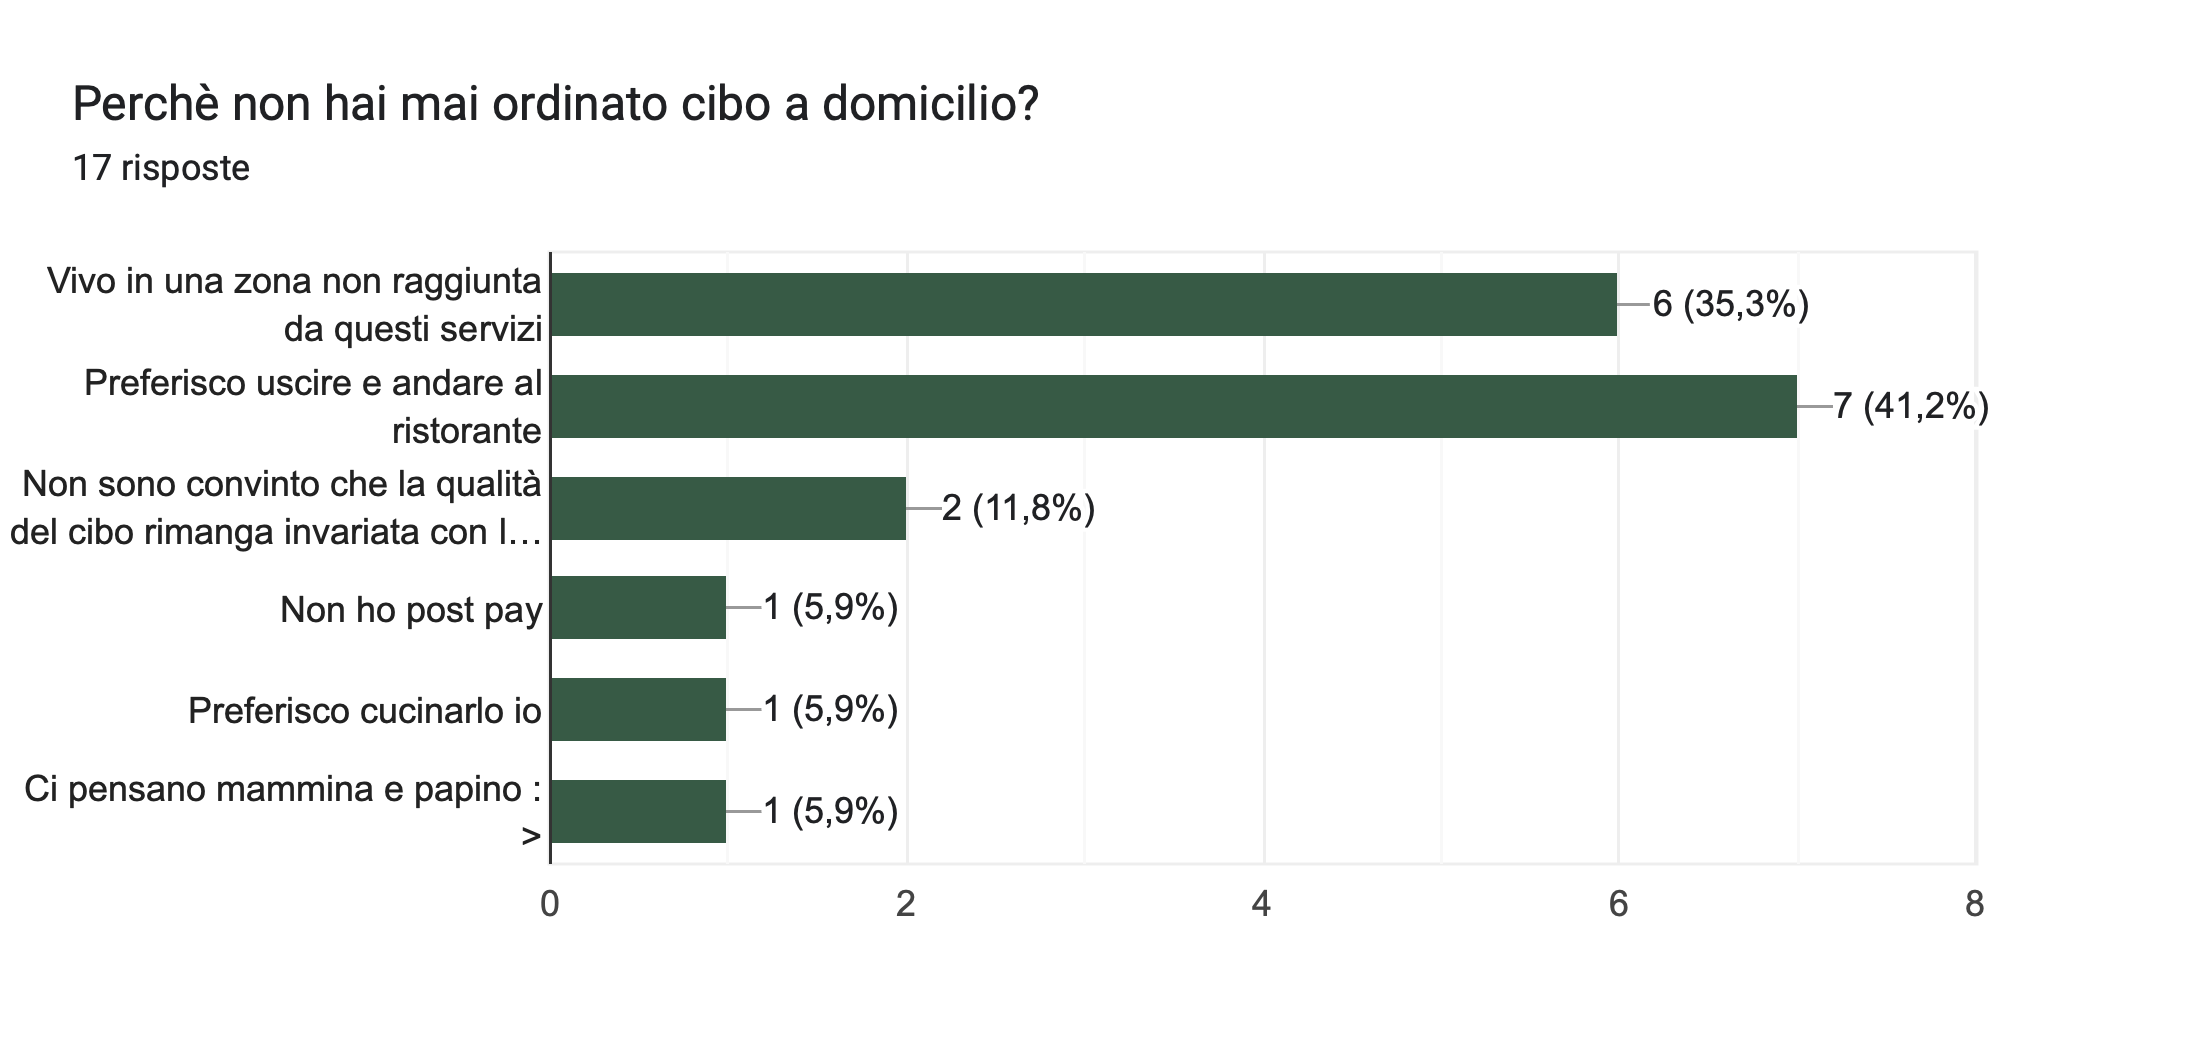
\includegraphics[width=\textwidth]{Data/Grafici/Perche_non_ordina.png}
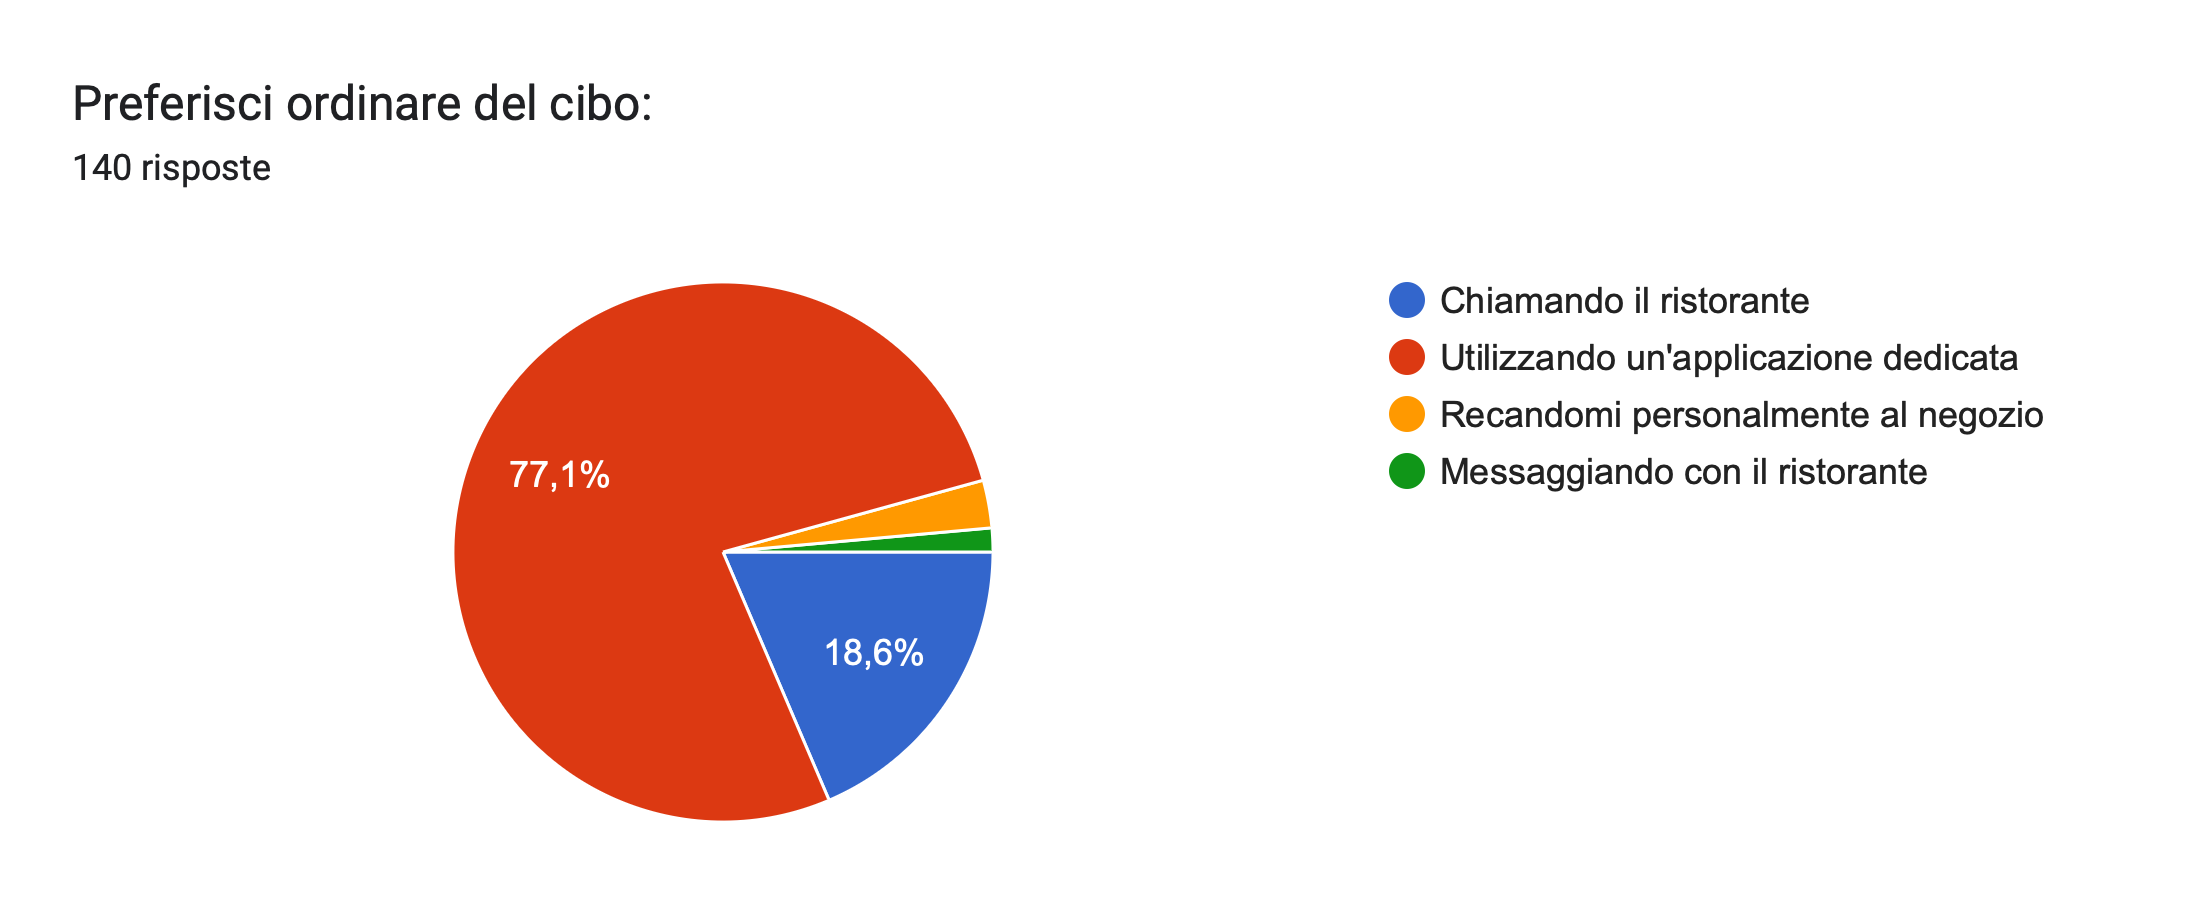
\includegraphics[width=\textwidth]{Data/Grafici/ordinare_cibo.png}
\par Abbiamo analizzato anche le risposte sulle percentuali dei metodi di consegna per capire quante persone usano le app di food delivery.\par \vspace{1cm}
\includegraphics[width=\textwidth]{Data/Grafici/Funzionalità_fondamentali.png}\par
Dalle risposte ottenute individuiamo quali sono le funzionalità che saltano subito alla vista degli utenti:
\par \begin{itemize}
    \item Tracciamento dell'ordine;
    \item Abbinamenti consigliati dal ristorante;
    \item Chattare con il rider;
    \item Visualizzare gli sconti disponibili;
\end{itemize}   \vspace{1cm} \par
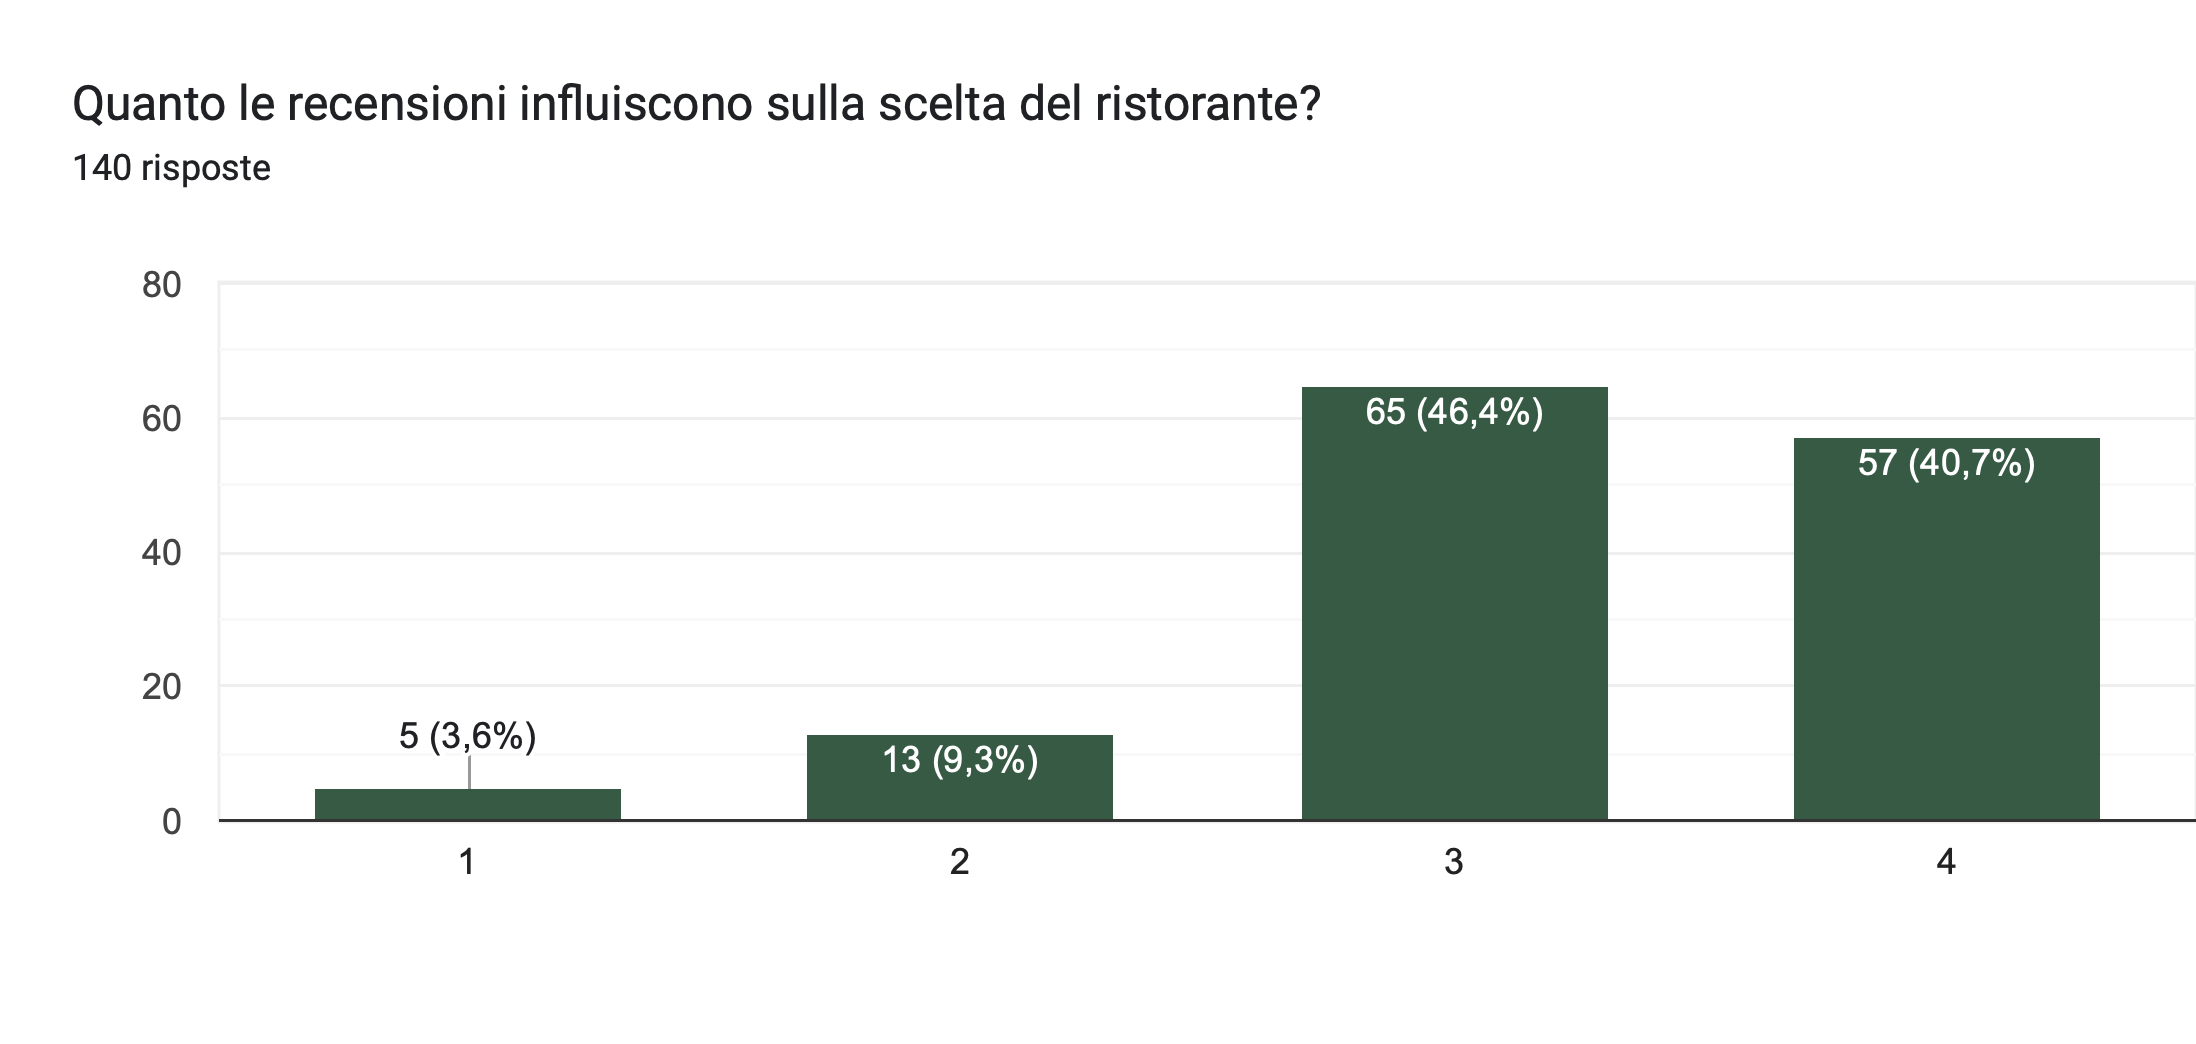
\includegraphics[width=\textwidth]{Data/Grafici/recensioni_influiscono.png}\par
Questa domanda l'abbiamo posta dopo un'accurata analasi dei competitor. Volevamo capire quanto le recensioni influiscano nella scelta di un ristorante, e decidere se implementare un sistema di recensioni semplice o completo come quello di UberEats.
    \par \vspace{1cm}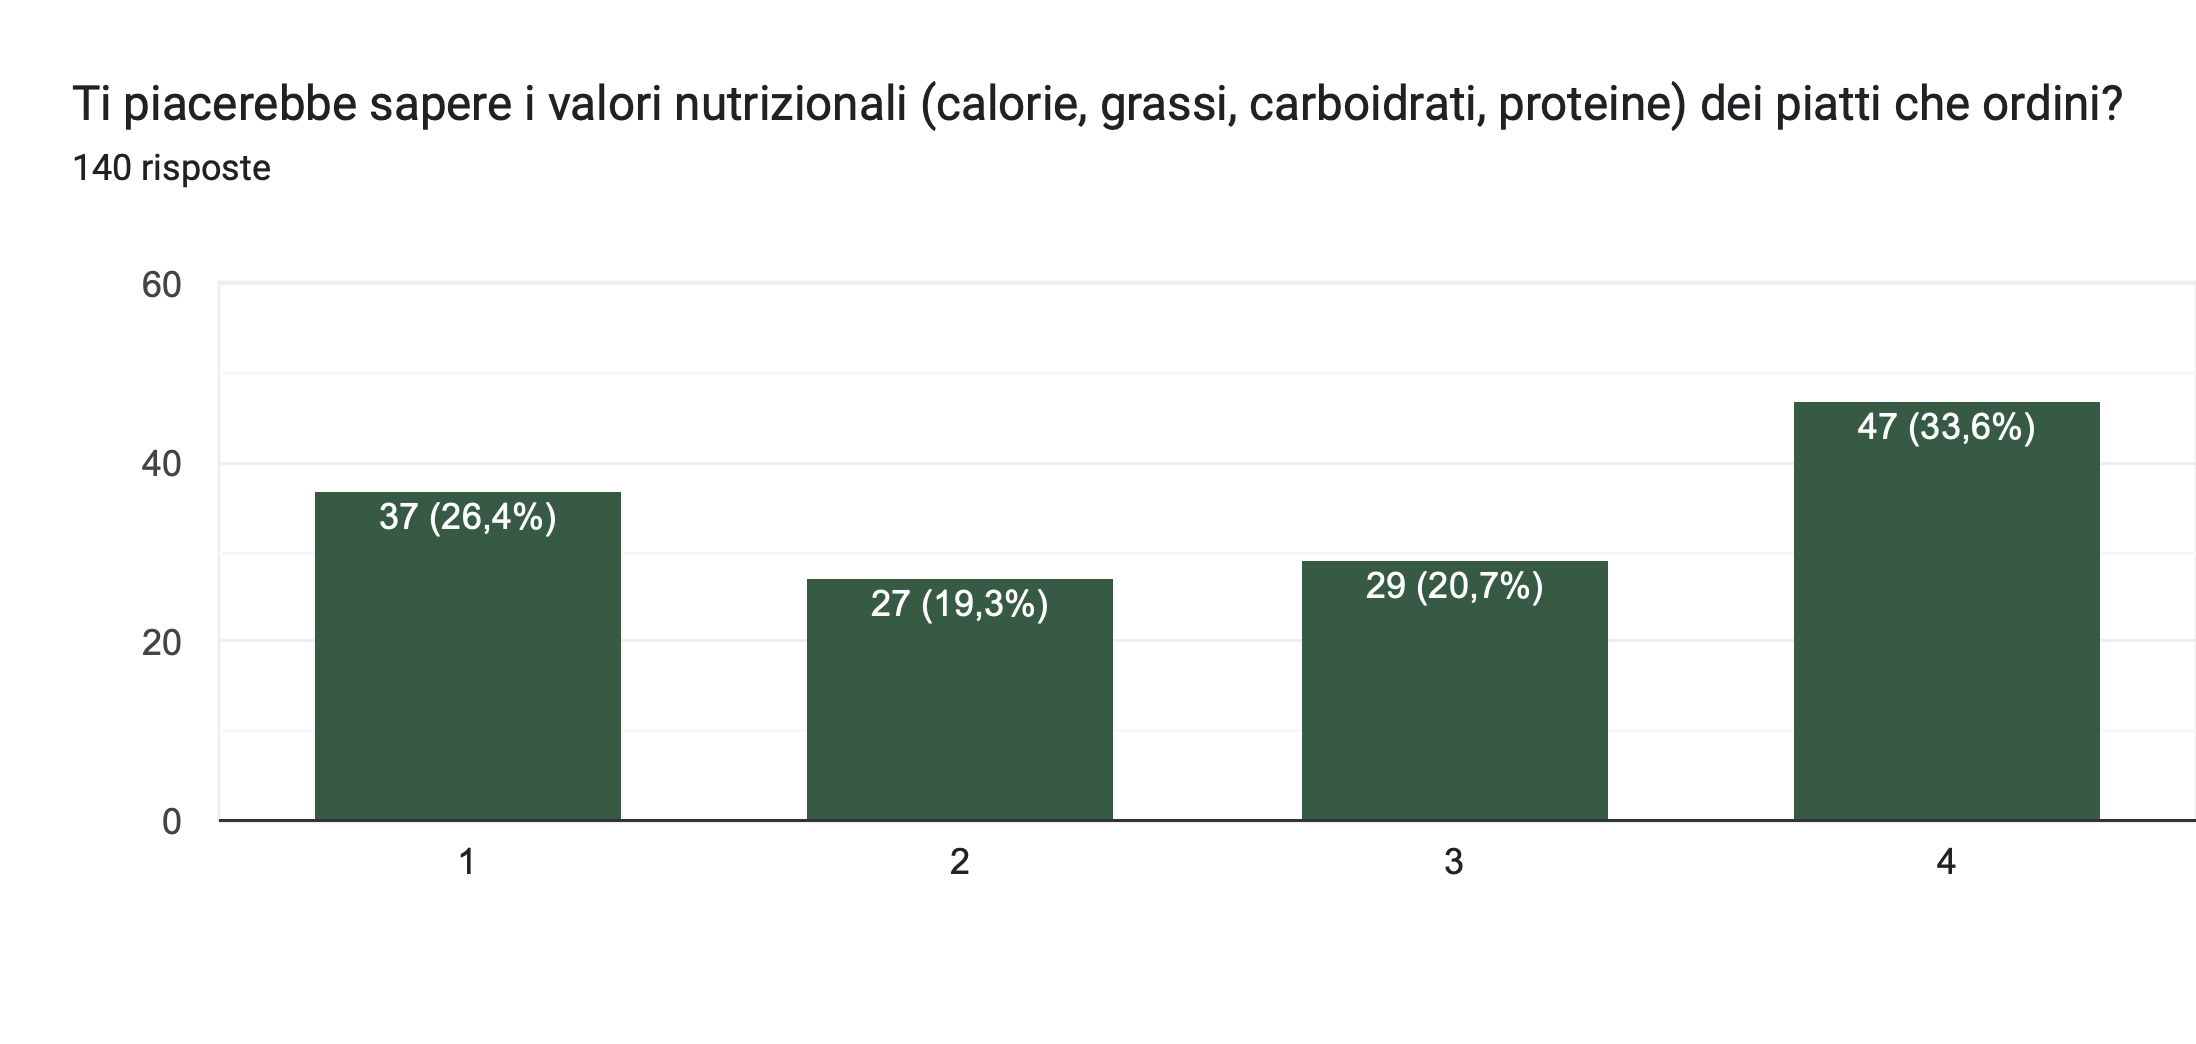
\includegraphics[width=\textwidth]{Data/Grafici/Valori_nutrizionali.png}\par
L'idea del controllo dei valori nutrizionali è emersa dalle interviste, essendo una funzionalità innovativa abbiamo inserito questa domanda nel questionario. È evidente che la maggioranza gradirebbe questa funzione, per questo è stata implementata nel prototipo.\par \vspace{1cm}
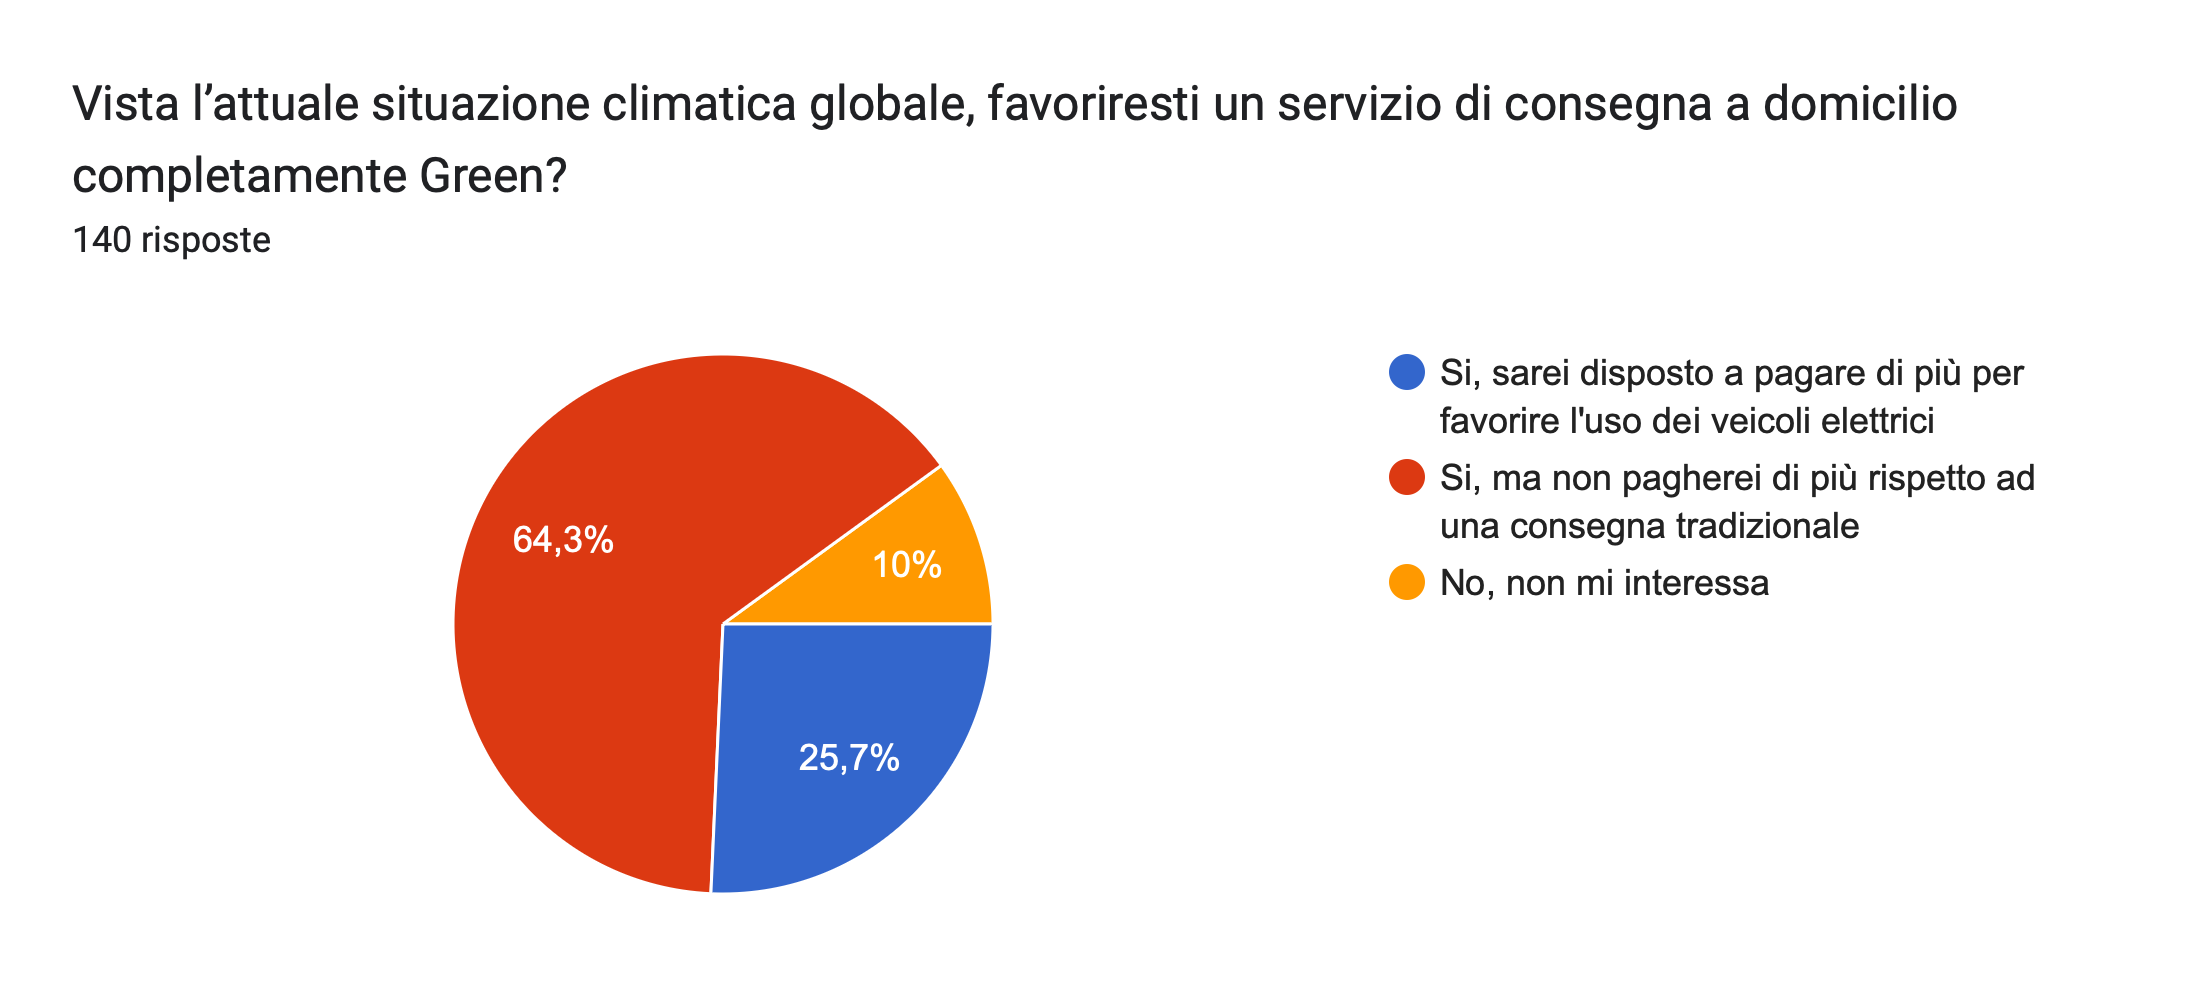
\includegraphics[width=\textwidth]{Data/Grafici/situazione_climatica.png}\par
Nelle interviste questa è stata la domanda più controversa e con più equilibrio tra i favorevoli e i contrari. Con il questionario ci siamo resi conto che questa idea non poteva essere implementata poichè solo il 25\% sarebbe disposto a pagare un sovrapprezzo. \par \vspace{1cm}
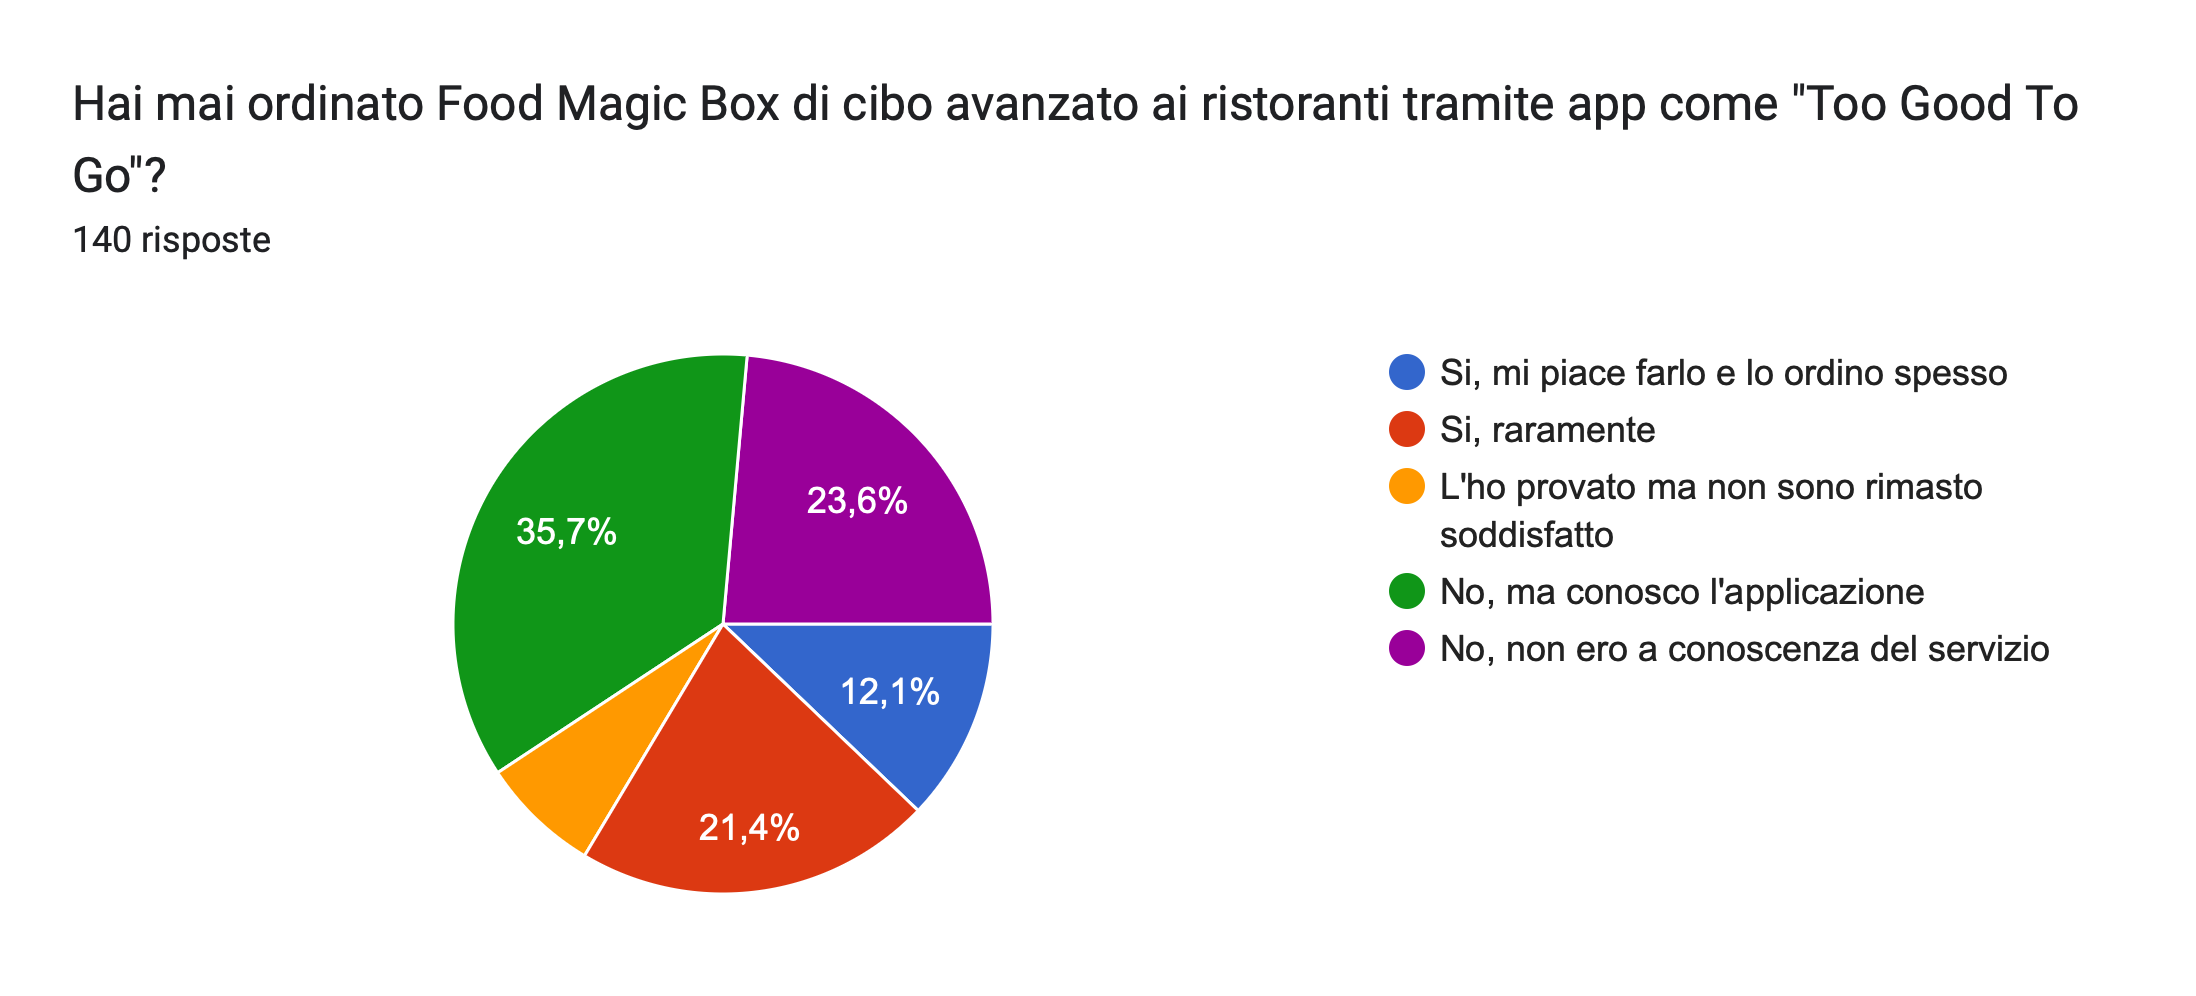
\includegraphics[width=\textwidth]{Data/Grafici/too_good_too_go.png}\par
.\par \vspace{1cm}
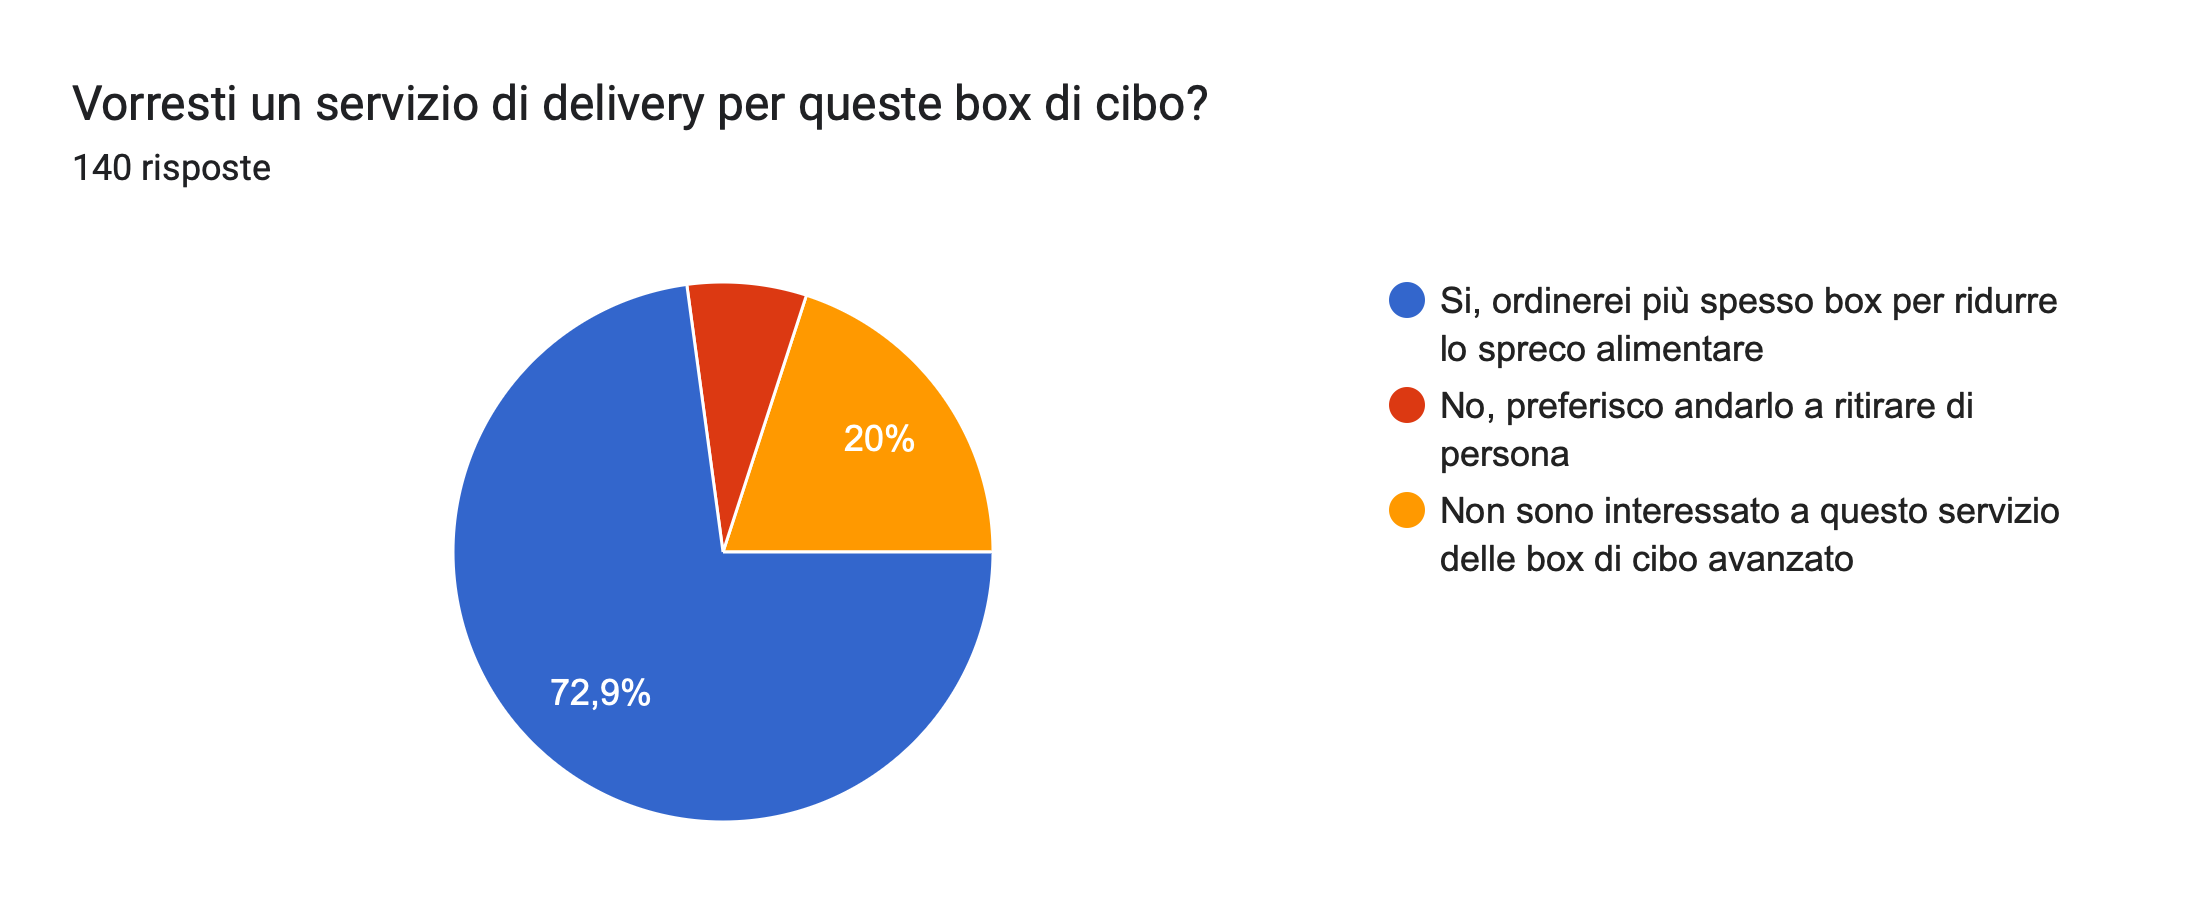
\includegraphics[width=\textwidth]{Data/Grafici/totg_delivery.png} \par
Dopo aver terminato le interviste e analizzato le risposte abbiamo notato che un ragazzo intervistato ha avuto l'idea della food magic box: una box contente l'invenduto di un ristorante ad un prezzo ridotto. È chiaro dai risultati dei questionari che questa tecnica per ridurre lo spreco alimentare non è diffusa. Analizzando l'app competitor "Too Good To Go" abbiamo notato che non offre il servizio di consegna a domicilio e chiedendo nei questionari è emerso che se questo fosse possibile la maggioranza inizirebbe ad ususfruire di questo servizio.
\begin{need}{}{theoexample}
    Dopo aver analizzato i risultati ottenuti dal questionario abbiamo riscontrato i seguenti need:
    \begin{enumerate}
        \item Risoluzione eventuali disguidi alla consegna.
        \item Combattere lo spreco alimentare.
        \item Visualizzazione in tempo reale della posizione del Rider.
        \item Avere la possibilità di recensire sia il ristorante, sia la pietanza singola.
        \item Avere a disposizione tutti i principali metodi di pagamento.
        \item Avere a disposizione un filtro per i \textit{valori nutrizionli} .
    \end{enumerate}
    \end{need}

    \vspace{1cm}
 \vspace{4cm}
\pagebreak
\section{Storyboard} \par
Le seguenti storyboard illustrano le principali task che sono state individuate:


\begin{figure}[htpb]

\begin{minipage}{0.40\textwidth}
    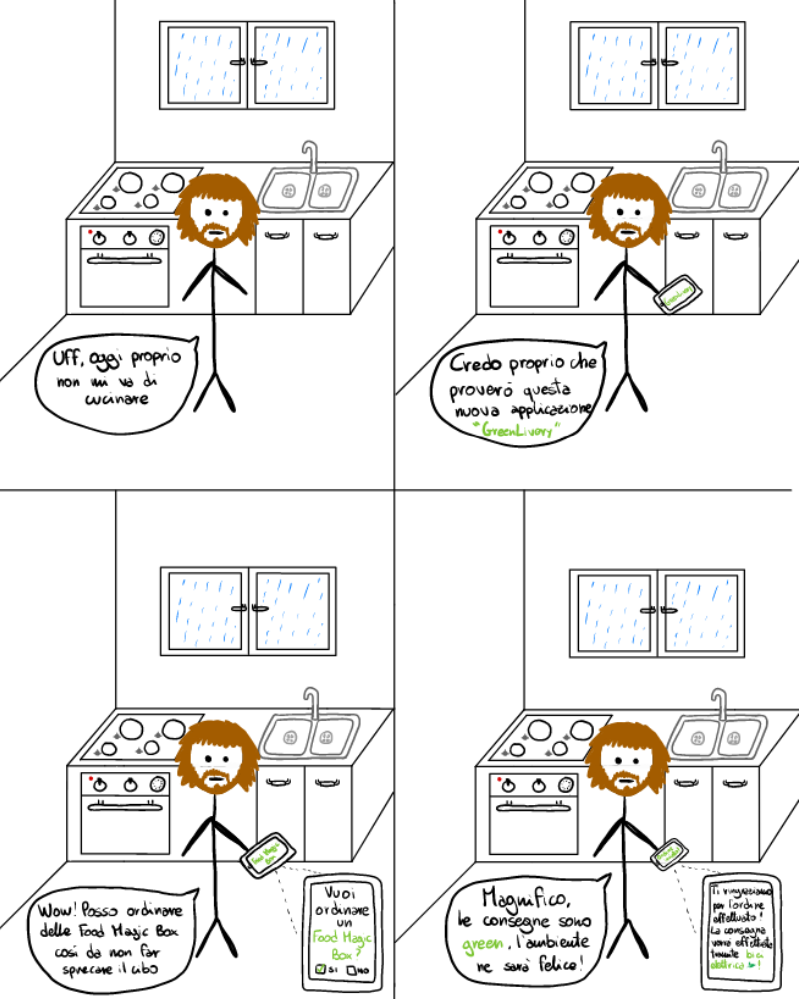
\includegraphics[width=\textwidth]{Data/StoryBoard/Effetuare_ordine.png}
    \caption[Prima figura]{Effettuare un ordine} \label{fig:1}
\end{minipage}
\hspace{2cm}
\begin{minipage}{0.40\textwidth}
    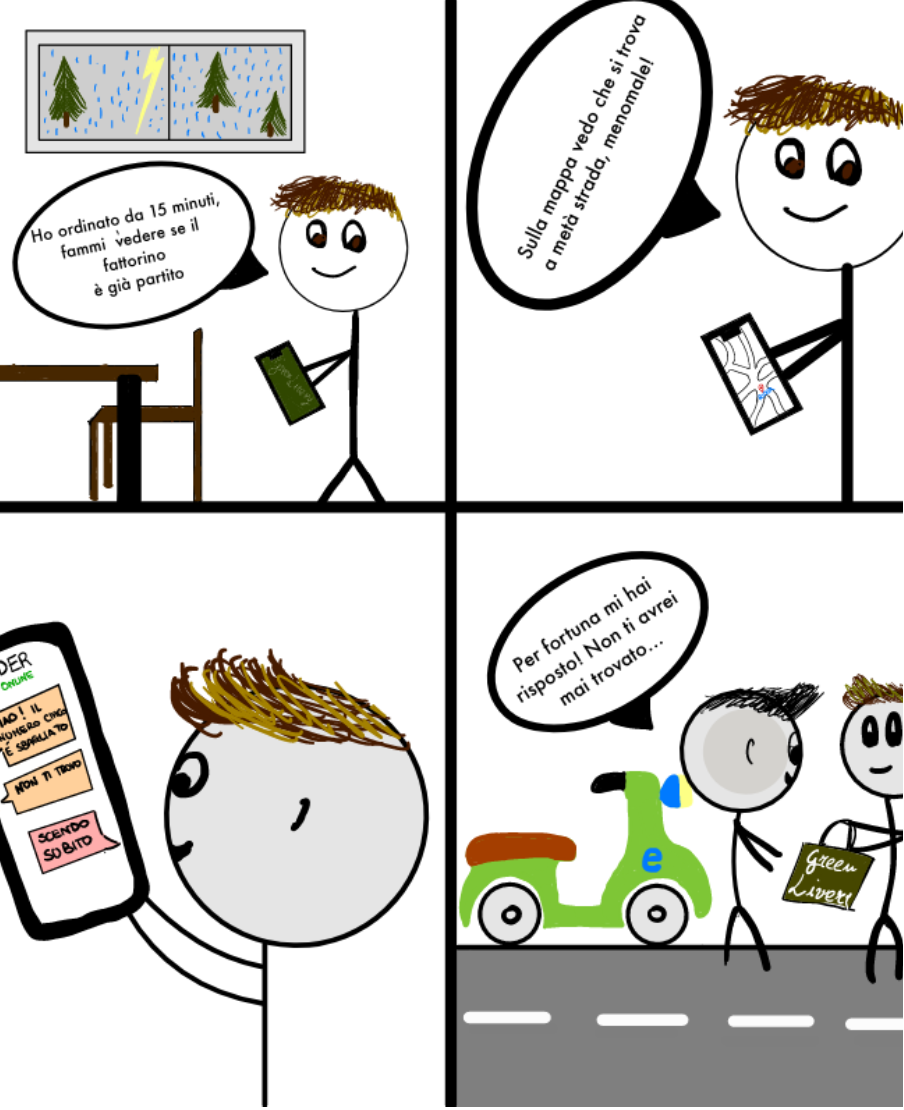
\includegraphics[width = \textwidth]{Data/StoryBoard/risoluzione disguidi alla cosegna.png}
    \caption[Seconda figura]{Usufruire dei servizi per avere una consegna precisa}\label{fig:2}
\end{minipage}
\begin{minipage}{0.40\textwidth}
    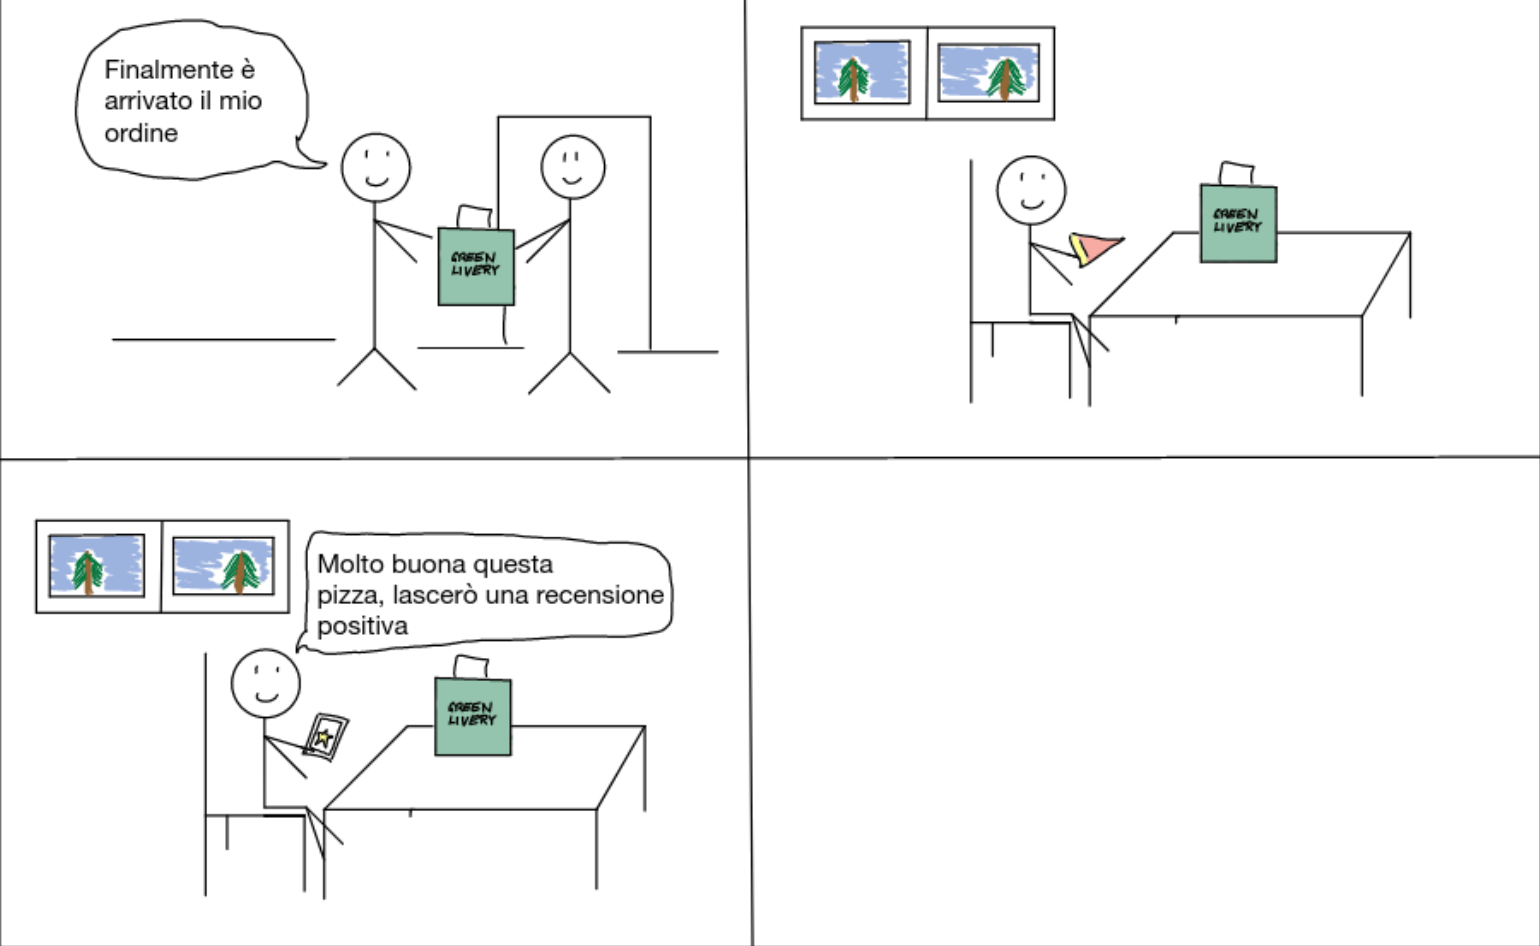
\includegraphics[width=\textwidth]{Data/StoryBoard/Recensione_ristorante.png}
    \caption[Terza figura]{Fornire valutazione ristorante e pietanza}\label{fig:3}
\end{minipage}
\hspace{2cm}
\begin{minipage}{0.40\textwidth}
    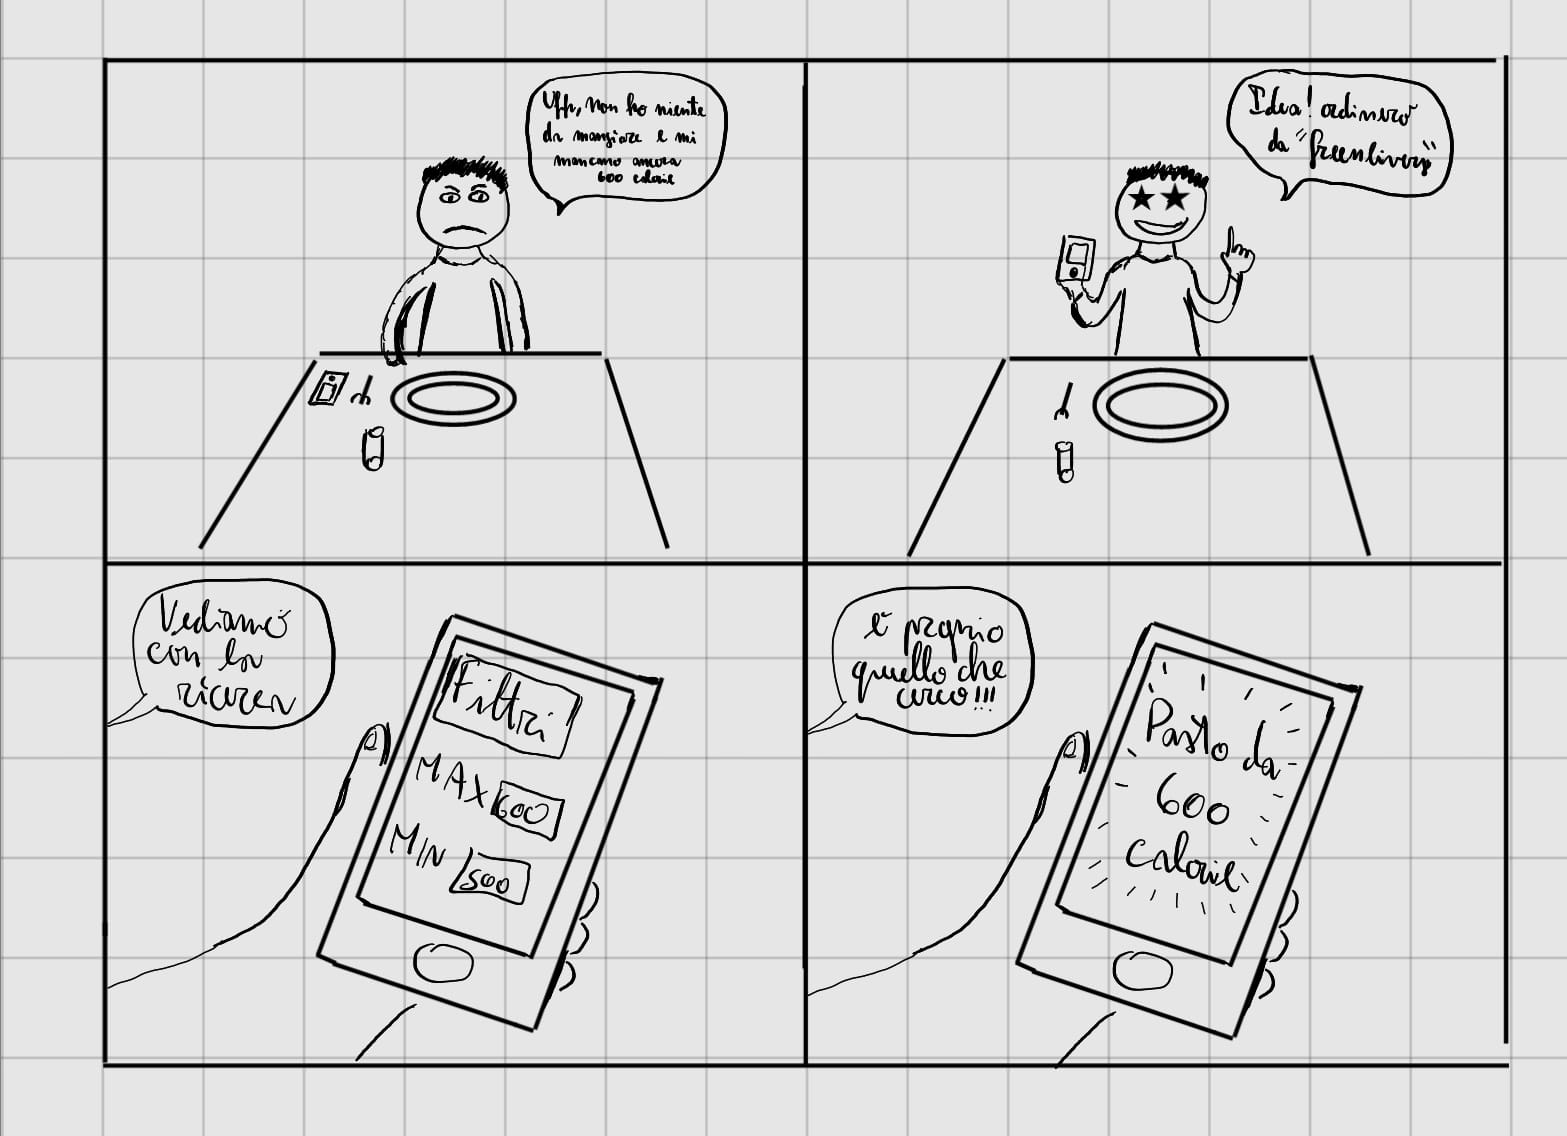
\includegraphics[width=\textwidth]{Data/StoryBoard/Filtro_calorie.jpeg}
    \caption[Quarta figura]{Usufruire del segna-calorie se si segue una dieta}\label{fig:4}
\end{minipage}
\end{figure}

\section{Prototipi}
    Ciascun task è stato testo da un gruppo di 8/10 persone e l'approccio al prototyping è stato di tipo evolutivo. Ad ogni iterazione,vengono proposte modifiche al fine di migliorare il prototipo e risolvere i problemi evidenziati nella versione precedente.\par
    
\begin{minipage}{0.40\textwidth}
    \addcontentsline{toc}{subsection}{\numberline{4.1}Versione 1}     
    \numberline{\fontsize{4mm}{1mm}\selectfont \textbf{4.1 Versione 1}}
    %scrivere qui 
    ciao
    \vspace{1cm}
    
    \addcontentsline{toc}{subsubsection}{\numberline{4.1.1}Versione 1 - Resoconto}
    \numberline{\fontsize{4mm}{1mm}\selectfont \textbf{4.1.1 Versione 1 - Resoconto}}
    %scrivere qui
    ciao
    \vspace{1cm}
\end{minipage}    
\hspace{2cm}
\begin{minipage}{0.40\textwidth}
    \addcontentsline{toc}{subsection}{\numberline{4.2}Versione 2}               
    \numberline{\fontsize{4mm}{1mm}\selectfont \textbf{4.2 Versione 2 }}
    %scrivere qui
    ciao
    \vspace{1cm}

    \addcontentsline{toc}{subsubsection}{\numberline{4.2.1}Versione 2 - Resoconto}
    \numberline{\fontsize{4mm}{1mm}\selectfont \textbf{4.2.1 Versione 2 - Resoconto}}
    %scrivere qui
    ciao
    \vspace{1cm}
\end{minipage}
\section{UserTest} \par\vspace{0.5cm}

\par Dopo aver terminato ciascuna versione del prototyping abbiamo effettuato un test di usabilità con diverse persone.
Il link per visualizzare tutti gli User Test è disponibile \textbf{\href{https://www.notion.so/User-Testing-03a9697158cb4f93b3439fe694f33ac9}{qui }.}
\section{Expert Evaluation}
\par Abbiamo successivamente effettuato un Expert Evaluation per testare l'usabilità del prototipo.
Il link per visualizzare l'Expert-Evaluation è disponibile \textbf{\href{https://www.notion.so/Expert-Evaluation-7bc49cae89414742a51b71f6faebecdd}{qui }.}

\vspace{1cm}

\end{document}